\documentclass[12pt,a4paper]{report}

\usepackage[utf8]{inputenc}
\usepackage[T1]{fontenc}
\usepackage[english]{babel}
\usepackage[a4paper,margin=25mm]{geometry}
\usepackage{amsmath,amssymb}
\usepackage{array,booktabs,tabularx}
\usepackage{graphicx}
\usepackage{float}
\usepackage{enumitem}
\usepackage{xurl}
\usepackage[hidelinks]{hyperref}

\setlength{\parskip}{0.5em}
\setlength{\parindent}{0pt}
\renewcommand{\arraystretch}{1.18}
\newcommand{\code}[1]{\texttt{#1}}

% Upload the comparison_charts folder beside this file in Overleaf.
\begin{document}

\setcounter{chapter}{5}
\chapter{EXPERIMENTAL SETUP AND RESULT ANALYSIS}

\section{Introduction}

This chapter describes the experimental configuration and comparative results of four autonomous network-defense approaches: GCN + SAC, GAT + DQN, GAT + PPO, and Attack Graph + Q-Learning. The experiments use a 50-node Fat-Tree-like network simulator, an eight-feature state for each node, eight defense actions, a common attack propagation function, and a shared reward implementation. The final comparison reports detection-style classification metrics, defense and containment rates, attack reduction, mean episode reward, and unnecessary isolation.

The results are the exact aggregate values currently stored in \code{comparison_results/comparison_metrics.csv} and used to produce the five charts in \code{comparison_charts/}. An important qualification is that the table is \textbf{not a verified, freshly paired four-model experiment}. The comparison runner reuses stored aggregate rows for GCN + SAC, GAT + DQN, and GAT + PPO when they already exist, while it trains and evaluates Attack Graph + Q-Learning. The first three results are therefore historical aggregates whose original invocation and scenario-level records are not present. The results are useful as descriptive project outputs, but they should not be used to claim statistical significance or a controlled paired-seed advantage.

\section{Experimental Environment}

\subsection{Hardware Configuration}

The active Windows host used for the latest Attack Graph + Q-Learning comparison was inspected directly. It has an AMD Ryzen 7 5825U processor with 8 physical cores and 16 logical processors, 16 GB installed RAM (approximately 13.84 GB reported as usable by Windows), and integrated AMD Radeon graphics. Windows reports 2 GB of adapter memory for the Radeon; because it is integrated graphics, this figure should not be interpreted as 2 GB of dedicated VRAM. The configured PyTorch package is the CPU build (2.11.0+cpu), reports no CUDA support, and therefore ran the latest Q-learning comparison on the CPU. These measurements describe the current host and latest Q-learning run. They cannot establish which hardware generated the older checkpoints or the previously stored GCN + SAC, GAT + DQN, and GAT + PPO aggregate results.

\begin{table}[htbp]
\centering
\caption{Measured hardware of the current host and latest Q-learning run.}
\begin{tabularx}{\textwidth}{>{\raggedright\arraybackslash}p{0.43\textwidth}X}
\toprule
\textbf{Item} & \textbf{Recorded information} \\
\midrule
Operating system & Windows 11 Home Single Language, version 10.0.26200 (build 26200) \\
Processor & AMD Ryzen 7 5825U with Radeon Graphics \\
CPU cores / logical processors & 8 physical cores / 16 logical processors \\
Installed / OS-usable memory & 16 GB installed / approximately 13.84 GB reported usable \\
Graphics adapter & AMD Radeon (TM) Graphics, integrated \\
Windows-reported adapter memory & 2 GB; shared/integrated graphics memory, not confirmed dedicated VRAM \\
Compute used by latest Q-learning run & CPU; PyTorch 2.11.0+cpu, CUDA unavailable \\
Older checkpoint and stored-baseline hardware & Cannot be inferred from current host measurements \\
\bottomrule
\end{tabularx}
\end{table}

The latest Q-learning run's host specifications are now reported from direct system inspection. For a reproducible four-model comparison, record the same hardware and software manifest at the time all four models are evaluated together; current host information cannot retrospectively identify the machine used to create older checkpoints or aggregates.

\subsection{Software Configuration}

The configured workspace interpreter inspected while preparing this chapter reports Python 3.14.0, PyTorch 2.11.0+cpu, PyTorch Geometric 2.7.0, NumPy 2.4.4, pandas 3.0.2, scikit-learn 1.8.0, and Matplotlib 3.10.8. These are the currently available environment versions, not a complete lockfile for the historical checkpoint runs; the project does not store a dependency lockfile or a run manifest with package versions.

The comparison runner selects CUDA if PyTorch reports it available and CPU otherwise. It seeds Python's \code{random}, NumPy, and PyTorch random generators with seed 42. CUDA-specific seeds and deterministic backend flags are not set. The attack simulator uses Python's \code{random} module, so its results depend on the exact random-number sequence and model execution order.

\subsection{Project Configuration Summary}

\begin{table}[htbp]
\centering
\caption{Default configuration used by the comparison runner.}
\begin{tabular}{lr}
\toprule
\textbf{Configuration} & \textbf{Value} \\
\midrule
Number of network nodes & 50 \\
Node features & 8 per node \\
Defense actions & 8 \\
Training episodes per newly trained policy & 5 \\
Training steps per episode & 20 maximum \\
Evaluation episodes & 50 \\
Evaluation steps per episode & 25 maximum \\
Random seed & 42 \\
GCN checkpoint path & \code{models/gcn\_pretrained.pt} \\
SAC checkpoint path & \code{models/sac\_agent.pt} \\
\bottomrule
\end{tabular}
\end{table}

\section{Dataset and Input Configuration}

\subsection{Dataset Description}

The project includes \code{combine.csv}, a flow-record CSV with a \code{Label} column, network-flow fields such as flow duration, forward and backward packet counts, packet and byte rates, TCP flags, and related traffic statistics. The local file contains approximately 2.2 million physical lines including its header. Dataset publisher, collection period, version, and original source URL are not recorded in the project, so this report does not assign it an external dataset name.

The project has a separate GCN-pretraining path that reads up to the first 10,000 rows, drops rows without a label, derives normalized features from flow fields, and constructs synthetic graph samples. The processor defaults to 2,000 graphs and splits the generated graph list by position into 80\% training and 20\% validation data. These are generated graph samples, not a direct row-wise 80/20 train/test split of the full CSV.

For the policy-comparison runs, the CSV is only loaded with \code{nrows=1} to verify that the file can be opened. The comparison episodes do \textbf{not} sample rows from \code{combine.csv}: the 50-node input features are initialized from the fixed feature table in \code{main.py}. Thus, the comparison environment is a simulator informed by project feature definitions, not a direct evaluation over held-out CSV flows. The \code{train\_size=0.8} argument passed to the CSV processor is not used to form a comparison train/test partition.

\subsection{Data Preprocessing}

The simulator's node input is an eight-element feature vector:

\begin{table}[htbp]
\centering
\caption{Node features used by the simulator.}
\begin{tabular}{cll}
\toprule
\textbf{Index} & \textbf{Feature} & \textbf{Representation} \\
\midrule
0 & Compromised & Binary indicator \\
1 & Risk score & Continuous value, nominally in [0, 1] \\
2 & Isolation status & Binary indicator \\
3 & Vulnerability score & Continuous value, nominally in [0, 1] \\
4 & Flow duration & Normalized continuous value \\
5 & Flow packets/s & Normalized continuous value \\
6 & Flow bytes/s & Normalized continuous value \\
7 & Node degree & Normalized topology degree \\
\bottomrule
\end{tabular}
\end{table}

The fixed simulator profile in \code{create\_network\_fat\_tree()} supplies the first seven values and updates degree from the generated topology. No CSV normalization or record-level split is applied to these simulator features. In the separate CSV graph-generation utility, duration, packet counts, and byte rate are min-max normalized from the selected input rows; flow labels are mapped to attack/non-benign flags when constructing synthetic GCN pretraining samples. These two pipelines should not be described as one shared preprocessing pipeline.

\section{Network Experimental Setup}

\subsection{Fat-Tree Topology}

The topology builder creates a manually adapted, 50-node Fat-Tree-like data-center network organized into three pods:

\begin{table}[htbp]
\centering
\caption{Node distribution in the simulated topology.}
\begin{tabular}{lr}
\toprule
\textbf{Network layer} & \textbf{Number of nodes} \\
\midrule
Core switches & 4 \\
Aggregation switches & 9 \\
Edge switches & 9 \\
Hosts & 28 \\
\textbf{Total} & \textbf{50} \\
\bottomrule
\end{tabular}
\end{table}

Each pod has aggregation and edge switches. Edge switches connect to aggregation switches within the pod and to a distribution of hosts; aggregation switches connect to core switches. Core switches are interconnected. The adjacency list is used for attack propagation and graph model input. It is a project-specific 50-node construction rather than a full textbook k-ary Fat Tree specification.

\subsection{Attack Scenario}

At the start of each episode, the same fixed 50-node feature profile is initialized. It includes compromised, risk, and isolation status as well as vulnerability and traffic features; the initialized profile has 21 compromised nodes. The attack routine selects the node with the greatest risk score as the attack target. If that node is isolated, the attack step ends. Otherwise, the target is compromised unless its selected action is \code{ISOLATE\_HOST} or \code{TERMINATE\_SESSION}.

The attacker then attempts to spread to the target's neighbors. The base probability is 0.5 and is modified by the neighbor's defense action: \code{MONITOR} 0.4, \code{RAISE\_ALERT} 0.3, \code{RATE\_LIMIT\_TRAFFIC} 0.2, \code{BLOCK\_DESTINATION\_PORT} 0.1, \code{BLOCK\_SOURCE\_IP} 0.05, and either isolation or session termination 0.0. \code{ALLOW\_TRAFFIC} leaves the base probability unchanged. Already isolated neighbors are skipped. The simulator marks nodes as compromised but has no compromise-recovery transition. An episode terminates early if every node is compromised; otherwise it runs up to its configured step limit.

\subsection{Defensive Actions}

All models use the same enum ordering and exactly eight actions:

\begin{table}[htbp]
\centering
\caption{Discrete defense actions used by all models.}
\begin{tabular}{rl}
\toprule
\textbf{ID} & \textbf{Action} \\
\midrule
0 & \code{ALLOW\_TRAFFIC} \\
1 & \code{MONITOR} \\
2 & \code{RAISE\_ALERT} \\
3 & \code{RATE\_LIMIT\_TRAFFIC} \\
4 & \code{BLOCK\_SOURCE\_IP} \\
5 & \code{BLOCK\_DESTINATION\_PORT} \\
6 & \code{ISOLATE\_HOST} \\
7 & \code{TERMINATE\_SESSION} \\
\bottomrule
\end{tabular}
\end{table}

For the discrete agents, an action is selected per node and mapped to its label. In the simulator, \code{ISOLATE\_HOST} and \code{TERMINATE\_SESSION} set the node's isolation feature. The action's effect on attack propagation is applied by the common \code{attack\_step()} function.

\section{Model Configuration}

\subsection{GCN + SAC}

The GCN has two graph-convolution layers: eight input features are mapped to a 64-unit hidden representation with ReLU, then to one sigmoid output per node. The output is used as the node risk prediction. During the policy comparison the GCN is loaded from \code{models/gcn\_pretrained.pt} and set to evaluation mode.

The SAC agent receives a flattened 450-value state: 50 nodes multiplied by eight node features plus one GCN risk prediction per node. It emits 50 continuous values in [0, 1], one per node. Each value is mapped to one of the eight actions using equal-width intervals. The SAC code uses actor and twin critic networks, a target critic, a replay buffer, entropy regularization, and automatic entropy-temperature adjustment. Its defaults include gamma 0.99, actor/critic learning rates 3e-4, temperature learning rate 1e-4, tau 0.005, and replay capacity 100,000. The supplied SAC checkpoint is loaded for evaluation; the comparison runner does not retrain it when a historical results row is already available.

\subsection{GAT + DQN}

GAT-DQN consumes the eight raw node features with graph connectivity. Its encoder uses two graph-attention layers with hidden size 64, four attention heads in the first layer, and one head in the second. A per-node Q-value head outputs eight action values. DQN uses epsilon-greedy action selection, experience replay, and an online/target network. Implemented defaults are gamma 0.99, learning rate 3e-4, batch size 32, capacity 10,000, epsilon 1.0, minimum epsilon 0.05, and multiplicative decay 0.995 per update. The existing comparison result is loaded from the aggregate artifact rather than re-created during the Q-learning run.

\subsection{GAT + PPO}

GAT-PPO uses the same two-layer GAT encoder and eight-action output space. Separate actor and critic heads produce per-node action logits and value estimates. Its implementation uses gamma 0.99, GAE lambda 0.95, clipping parameter 0.2, learning rate 3e-4, entropy coefficient 0.01, and value coefficient 0.5. Training stores sampled actions, log probabilities, and values for policy updates. The aggregate comparison result is a stored result and was not freshly reproduced as part of the latest Q-learning-only evaluation.

\subsection{Attack Graph + Q-Learning}

\code{build\_attack\_graph()} derives an attack graph from the same current simulator adjacency list and node features. Nodes retain identity, compromise, risk, vulnerability, isolation, and the original feature vector. Edges encode network reachability after isolated nodes are excluded. The graph additionally calculates compromised-neighbor count, the number of reachable vulnerable nodes within two hops, shortest-path distance from the nearest compromised source, and a graph risk score:

\begin{equation}
R_g(v)=\operatorname{clip}\left(0.5R(v)+0.3V(v)+0.2E_2(v),0,1\right),
\end{equation}

where $R(v)$ is the simulator risk, $V(v)$ is vulnerability, and $E_2(v)$ is the mean vulnerability among the node's one- and two-hop reachable nodes. The \code{discretize\_attack\_graph\_state()} function builds one tabular key per node containing node identity, compromise bit, five-bin graph risk, isolation bit, four-bin vulnerability, 0/1/2+ reachable-vulnerable count, 0/1/2+ compromised-neighbor count, and path distance 0/1/2/3+ or unreachable. This retains node-specific and graph-derived context instead of reducing the network to one global scalar.

\code{AttackGraphQLearningAgent} has a Q-table with eight values per encountered node-state. It applies epsilon-greedy exploration and the standard update:

\begin{equation}
Q(s,a)\leftarrow Q(s,a)+\alpha\left[r+\gamma\max_{a'}Q(s',a')-Q(s,a)\right].
\end{equation}

The configured parameters are alpha 0.2, gamma 0.95, initial epsilon 1.0, minimum epsilon 0.05, and epsilon decay 0.97 once after each training episode. The Q-table is initialized empty and is trained online; it is not pretrained from \code{combine.csv} and uses no neural network. At each transition the shared network reward is applied to each node's state-action update. This is a node-wise tabular approximation to the joint 50-node decision problem, not a joint Q-table over all simultaneous network actions.

\section{Training Configuration}

The comparison runner's default budget is five training episodes with up to 20 steps per episode, followed by 50 separate evaluation episodes with up to 25 steps each. Evaluation uses deterministic action selection for the neural policies and greedy (non-exploratory) selection for Q-learning. Early termination occurs if every network node is compromised. The Q-learning trainer prints episode reward, per-step average reward, epsilon, and number of learned table states.

In the latest Q-learning run, training episode rewards were approximately -64.040, -60.079, -64.577, -68.195, and -61.595. Corresponding average rewards per step were approximately -3.202, -3.004, -3.229, -3.410, and -3.080; epsilon decreased from 1.0 to 0.859. These values are training diagnostics, not evaluation results and not a fabricated learning curve. Five episodes are a small budget for tabular reinforcement learning; they demonstrate that table updates occur but are insufficient to establish convergence.

The GCN checkpoint is a separate pretrained artifact. The GCN training script describes pretraining on generated graphs from CSV-derived flows and the command-line default is 20 epochs; the training function's own default is 100 epochs. The precise epoch count and provenance of the checked-in checkpoint are not recorded. The GAT policies are trained for five episodes only when the comparison runner finds their results missing; because aggregate rows already existed, that path was not run during the latest Q-only evaluation.

\section{Experimental Procedure}

The comparison workflow is:
\begin{enumerate}[leftmargin=2em]
  \item Seed Python \code{random}, NumPy, and PyTorch with 42 and select the available compute device.
  \item Read one row from \code{combine.csv} to validate that the dataset file is accessible. This is not used to construct episode features.
  \item Load the GCN checkpoint and enter evaluation mode.
  \item Read previously stored aggregate results for models already present in the comparison CSV/JSON.
  \item Initialize a fresh Attack Graph + Q-Learning agent, train it for five episodes using the fixed Fat Tree simulator, common attack transition, and common reward function.
  \item Reset the random seeds and evaluate the learned Q-table greedily over 50 episodes, with up to 25 steps per episode.
  \item Aggregate per-node detection labels/scores, defense/containment events, compromise counts, episode reward, unnecessary isolation, and action counts.
  \item Append the Q-learning result, preserve existing baseline aggregates, and export the CSV, JSON, and comparison plot.
\end{enumerate}

Although the same simulator implementation and default episode budgets are specified in the runner, the present aggregate table is mixed-vintage. Existing result rows are reused rather than all four agents being evaluated on common saved scenario seeds. The current workflow therefore does not support a strict same-scenario paired comparison.

\section{Evaluation Metrics}

The runner uses scikit-learn for accuracy, precision, recall, F1, and ROC-AUC. The definitions below follow the current code exactly. During each step, the target label for a node is positive if it was already compromised or its pre-action simulator risk is at least 0.6. A predicted positive is any selected action other than \code{ALLOW\_TRAFFIC}. Consequently, the reported detection metrics measure action/non-action agreement with this simulator heuristic; they are not an independent test of the GCN's classification accuracy against held-out CSV ground truth.

\begin{table}[htbp]
\centering
\caption{Evaluation metrics and implementation definitions.}
\small
\begin{tabularx}{\textwidth}{>{\raggedright\arraybackslash}p{0.25\textwidth}X}
\toprule
\textbf{Metric} & \textbf{Current calculation/definition} \\
\midrule
Accuracy & Correct predicted node labels divided by all node labels. \\
Precision & True positive action flags divided by all positive action flags; zero-division returns 0. \\
Recall & True positive action flags divided by all positive heuristic targets; zero-division returns 0. \\
F1 & Harmonic mean of precision and recall. \\
ROC-AUC & Area under ROC computed from model-specific action scores. Scores are transformed policy outputs, not calibrated probabilities. \\
Defense Success Rate & Successful defensive actions divided by all non-ALLOW defensive actions. A success requires a previously high-risk node to remain clean, or a compromised node to be isolated by an isolation action. \\
Attack Containment Rate & Steps with an attack opportunity and no newly compromised nodes divided by attack-opportunity steps. An opportunity occurs when the highest-risk node is not already isolated. \\
Attack Reduction Rate & $100\times(\text{initial compromised count}-\text{final compromised count})/\max(1,\text{initial compromised count})$, aggregated over episodes. \\
Average Episode Reward & Arithmetic mean of total shared reward per evaluation episode. \\
Unnecessary Isolation Rate & Healthy-node isolation actions divided by all isolation actions, multiplied by 100. Isolation actions are \code{ISOLATE\_HOST} and \code{TERMINATE\_SESSION}. The numerator is a subset of the denominator under the current implementation. \\
\bottomrule
\end{tabularx}
\end{table}

The shared reward depends on changes in compromised nodes, changes in isolated compromised and healthy nodes, mean risk reduction, bonuses for no new compromise or a clean network, action operating costs, and action penalties on nodes that are not high risk. Per-node totals are normalized by the node count and the final reward is clipped to [-100, 100]. For action label $a$, the implemented costs are: allow 0, monitor 0.5, alert 1, rate limit 2, source/port block 4, isolate 8, and terminate 10. Low-risk rate-limit/alert actions incur penalty 2; low-risk source/port blocks incur penalty 4; low-risk isolation/termination incurs penalty 8.

For the score used by ROC-AUC, SAC transforms its continuous output as $\max(0,(a-0.125)/0.875)$; DQN and Q-learning use one minus the softmax probability assigned to action 0; PPO uses one minus the policy probability assigned to action 0. Since these scores have different constructions, ROC-AUC differences should be interpreted cautiously.

\section{Experimental Results}

The following table reproduces the current aggregate results. Percent metrics are displayed as percentages, converting the stored [0, 1] detection values by multiplying by 100. Reward is dimensionless and is shown on its native scale.

\begin{table}[htbp]
\centering
\caption{Current aggregate comparison results.}
\scriptsize
\resizebox{\textwidth}{!}{%
\begin{tabular}{lrrrrrrrrrr}
\toprule
\textbf{Model} & \textbf{Accuracy (\%)} & \textbf{Precision (\%)} & \textbf{Recall (\%)} & \textbf{F1 (\%)} & \textbf{ROC-AUC (\%)} & \textbf{Defense success (\%)} & \textbf{Containment (\%)} & \textbf{Attack reduction (\%)} & \textbf{Average reward} & \textbf{Unnecessary isolation (\%)} \\
\midrule
GCN + SAC & 77.616 & 77.159 & 100.000 & 87.107 & 94.909 & 24.852 & 91.250 & -23.810 & 17.538 & 0.000 \\
GAT + DQN & 75.288 & 75.288 & 100.000 & 85.902 & 67.415 & 24.486 & 89.333 & -23.810 & -31.142 & 0.000 \\
GAT + PPO & 75.125 & 75.125 & 100.000 & 85.796 & 42.620 & 24.533 & 88.083 & -23.810 & -48.036 & 0.000 \\
Attack Graph + Q-Learning & 67.426 & 73.522 & 87.339 & 79.837 & 47.065 & 42.404 & 99.834 & -17.429 & -79.482 & 46.124 \\
\bottomrule
\end{tabular}%
}
\end{table}

\subsection{Detection Results}

GCN + SAC has the highest accuracy (77.616\%), F1 (87.107\%), and ROC-AUC (94.909\%) in the current table. All three existing neural-policy rows have 100\% recall under the current target/action definitions. Attack Graph + Q-Learning reports accuracy 67.426\%, precision 73.522\%, recall 87.339\%, F1 79.837\%, and ROC-AUC 47.065\%. These are action-based simulator metrics and not held-out data classification results.

\subsection{Defense Results}

Attack Graph + Q-Learning has the highest reported defense success rate (42.404\%) and attack containment rate (99.834\%). These rates coexist with its high unnecessary-isolation rate (46.124\%) and low average reward (-79.482), showing that aggressive defenses can register containment while incurring substantial operational penalties. GCN + SAC has 91.250\% containment with 0\% unnecessary isolation in the stored aggregate.

\subsection{RL Results}

The average episode rewards are 17.538 for GCN + SAC, -31.142 for GAT + DQN, -48.036 for GAT + PPO, and -79.482 for Attack Graph + Q-Learning. The Q-learning result is poor on the shared reward scale despite high containment. Its training episode totals also remain negative. No trend has been forced or smoothed; the values reflect the executed implementation and stored aggregates.

\section{Graphical Result Analysis}

The following figures use only the aggregate values in Section 6.9. They do not represent episode-level traces or training curves. Upload the five PNG files while preserving the \code{comparison\_charts/} directory structure in Overleaf.

\begin{figure}[htbp]
\centering
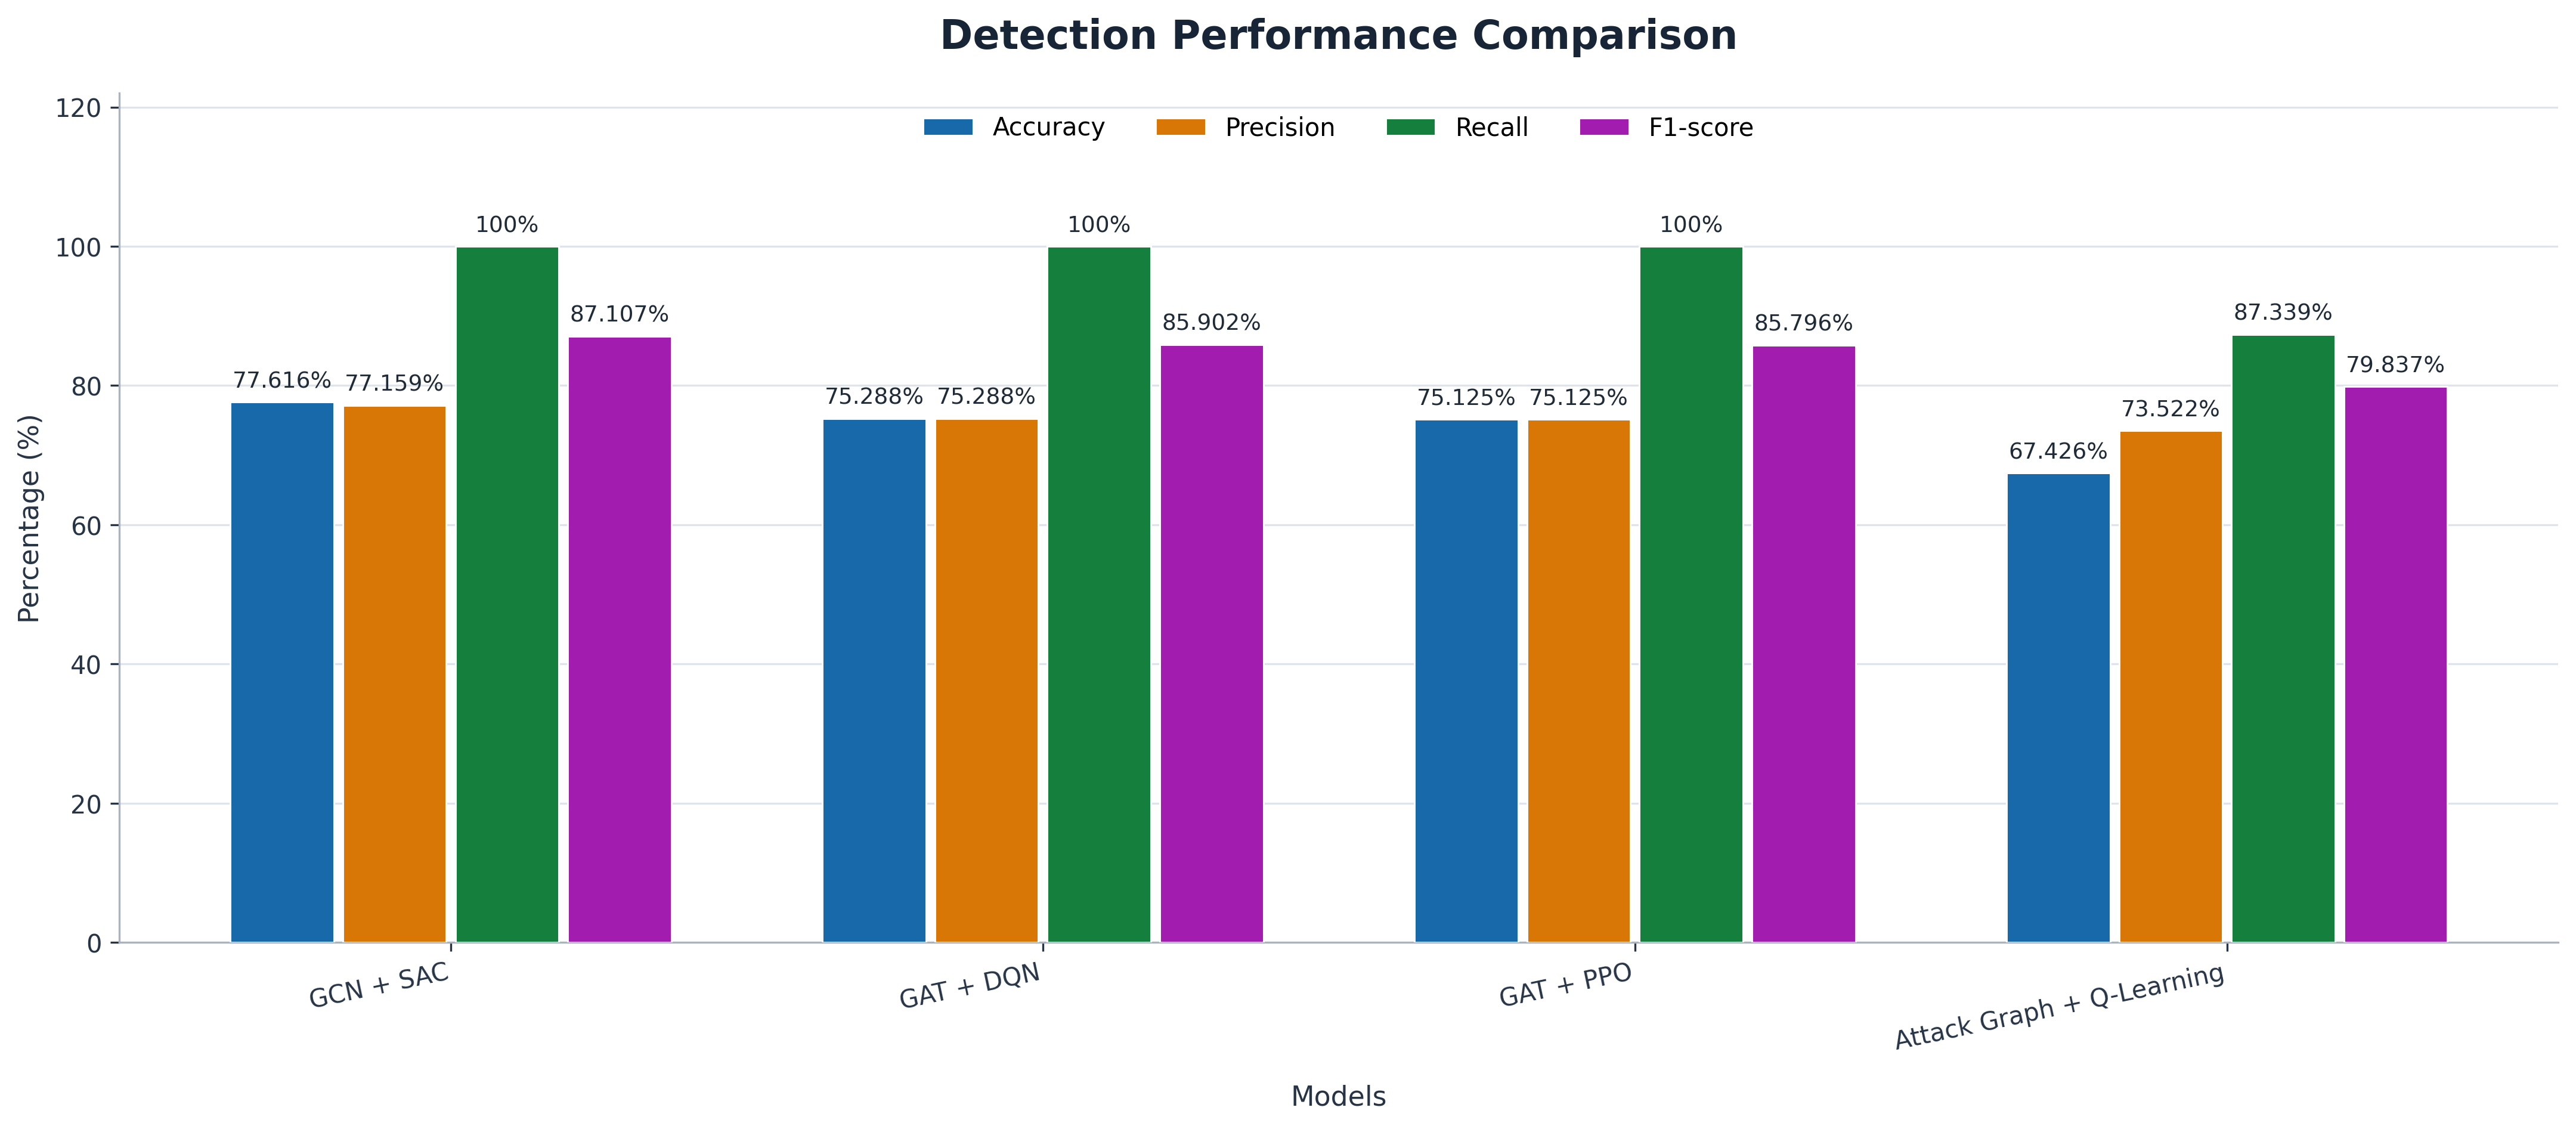
\includegraphics[width=0.98\textwidth]{comparison_charts/01_detection_performance.png}
\caption{Accuracy, precision, recall, and F1-score for the four models.}
\label{fig:detection-performance}
\end{figure}

\begin{figure}[htbp]
\centering
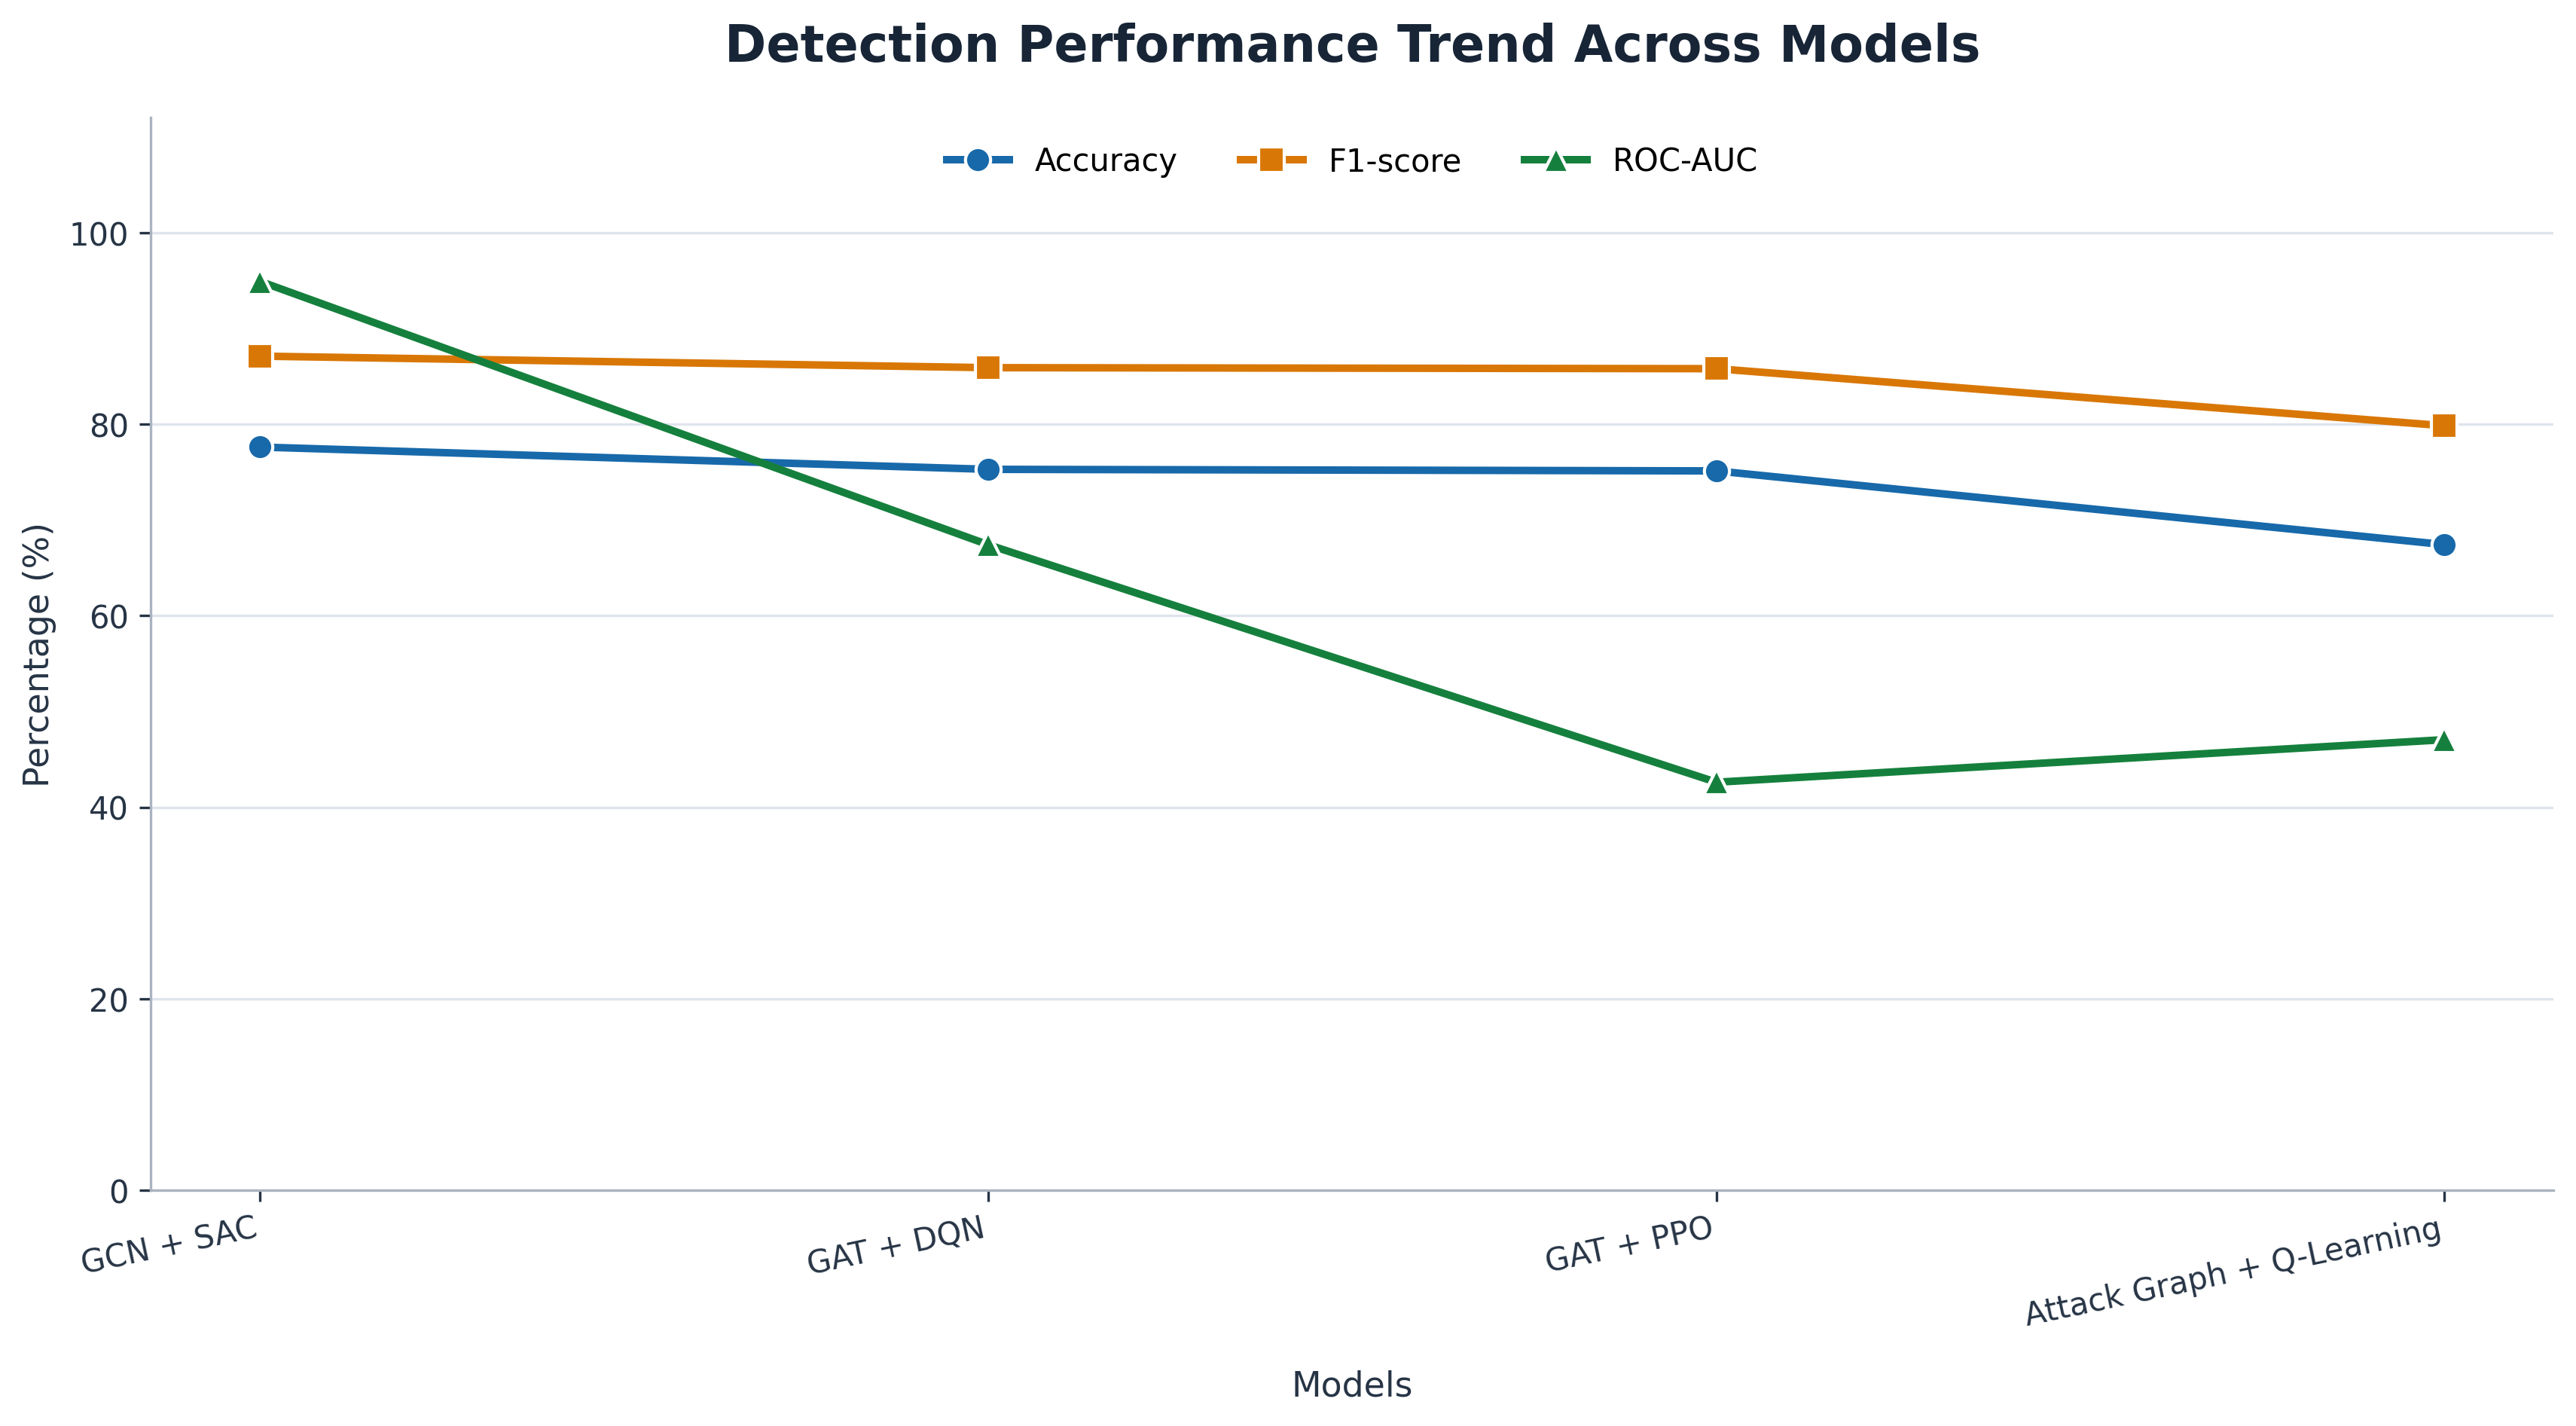
\includegraphics[width=0.98\textwidth]{comparison_charts/02_model_performance_line.png}
\caption{Aggregate accuracy, F1-score, and ROC-AUC compared across models.}
\label{fig:detection-metric-comparison}
\end{figure}

\begin{figure}[htbp]
\centering
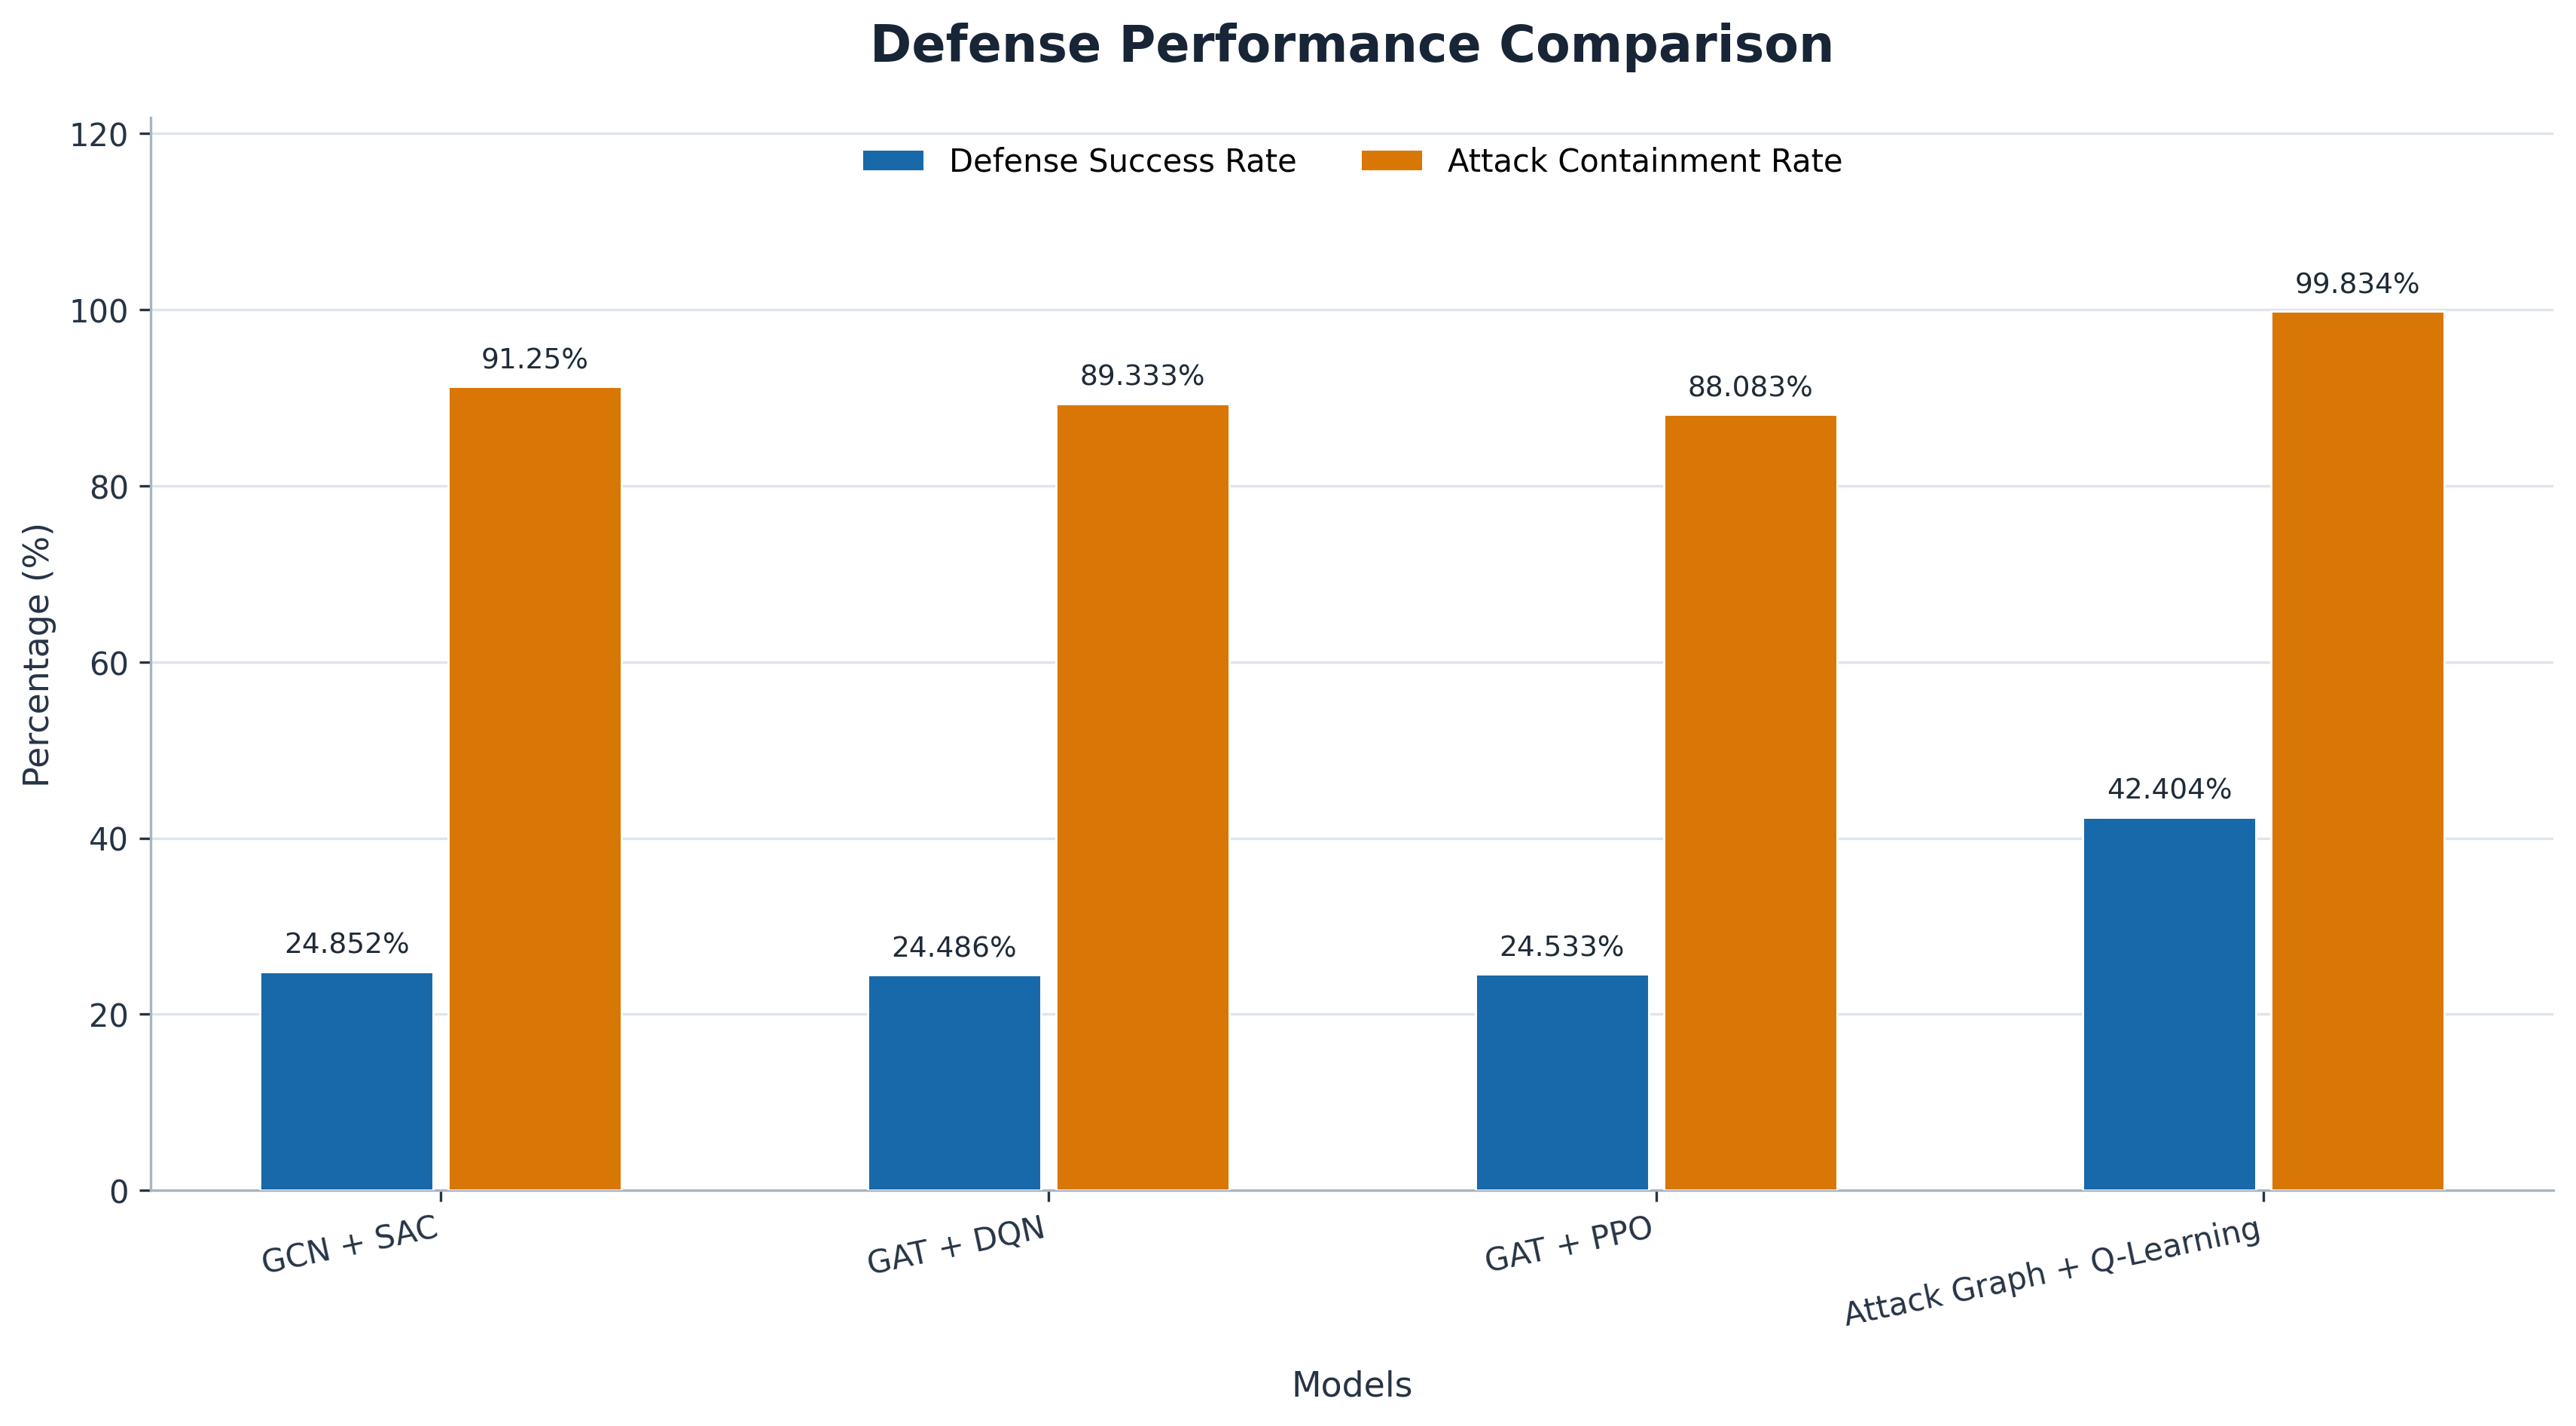
\includegraphics[width=0.98\textwidth]{comparison_charts/03_defense_performance.png}
\caption{Defense success and attack containment rates by model.}
\label{fig:defense-performance}
\end{figure}

\begin{figure}[htbp]
\centering
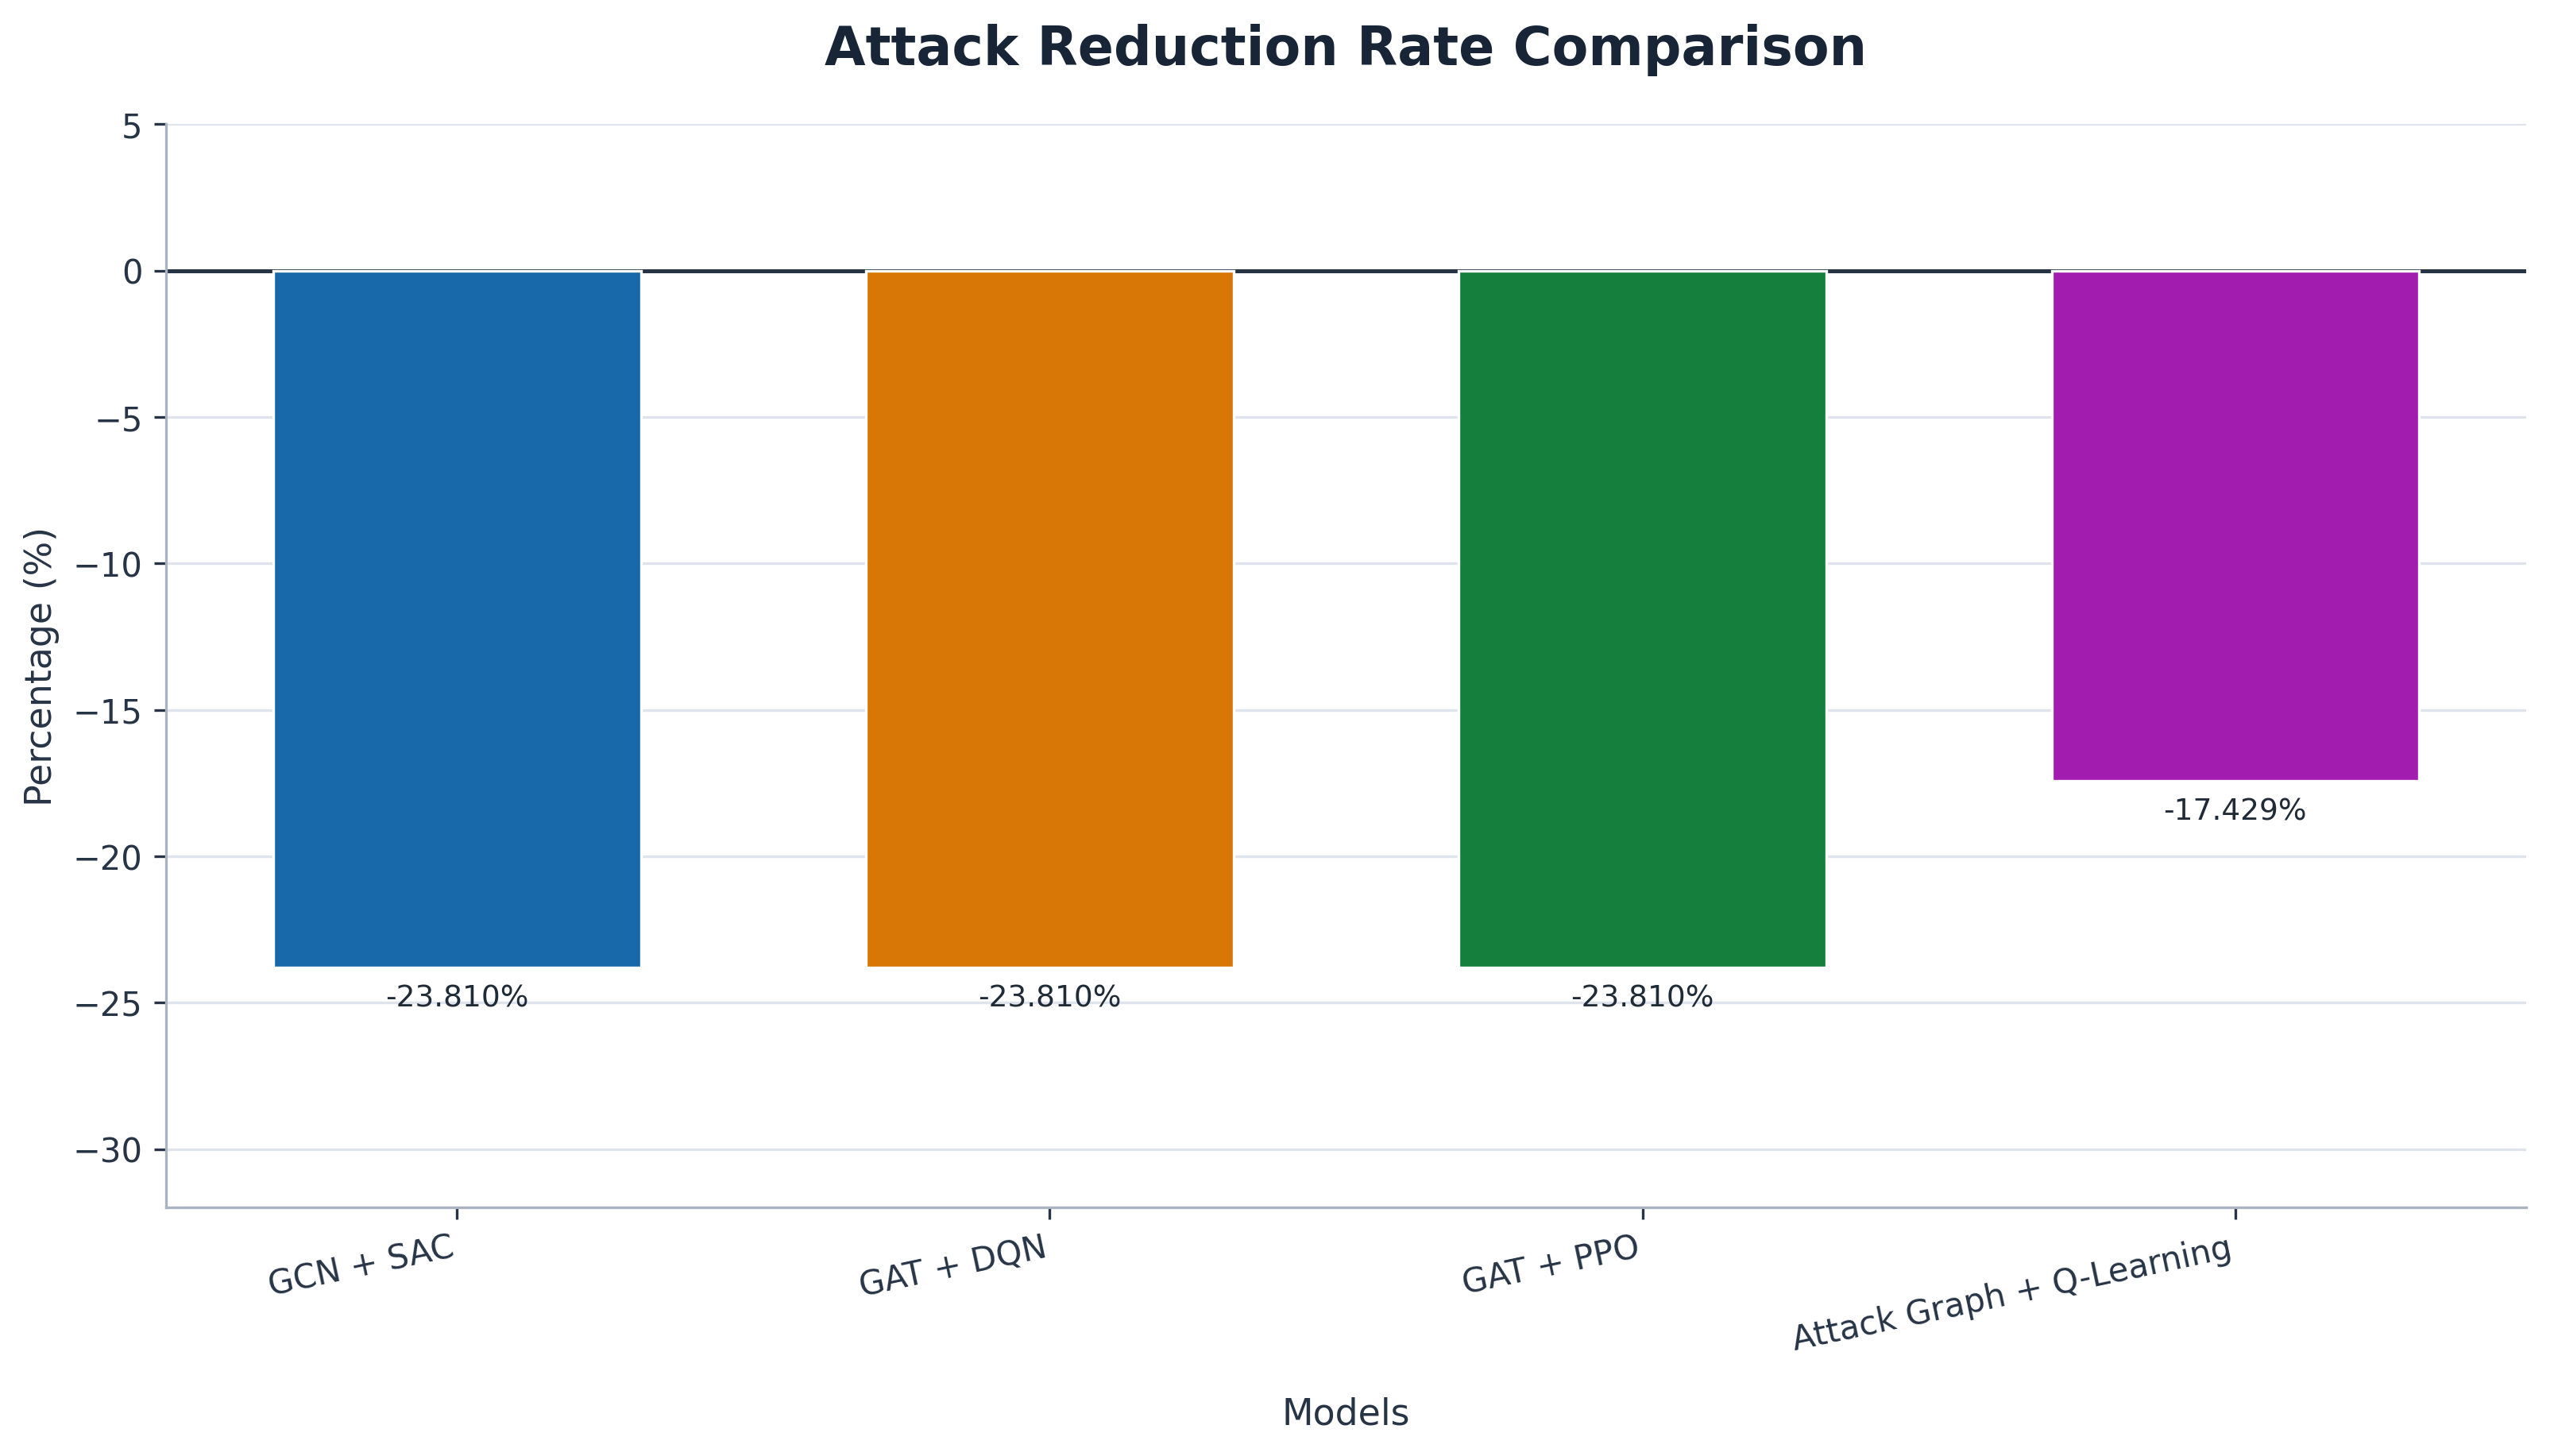
\includegraphics[width=0.98\textwidth]{comparison_charts/04_attack_reduction.png}
\caption{Attack reduction rates, retaining negative values.}
\label{fig:attack-reduction}
\end{figure}

\begin{figure}[htbp]
\centering
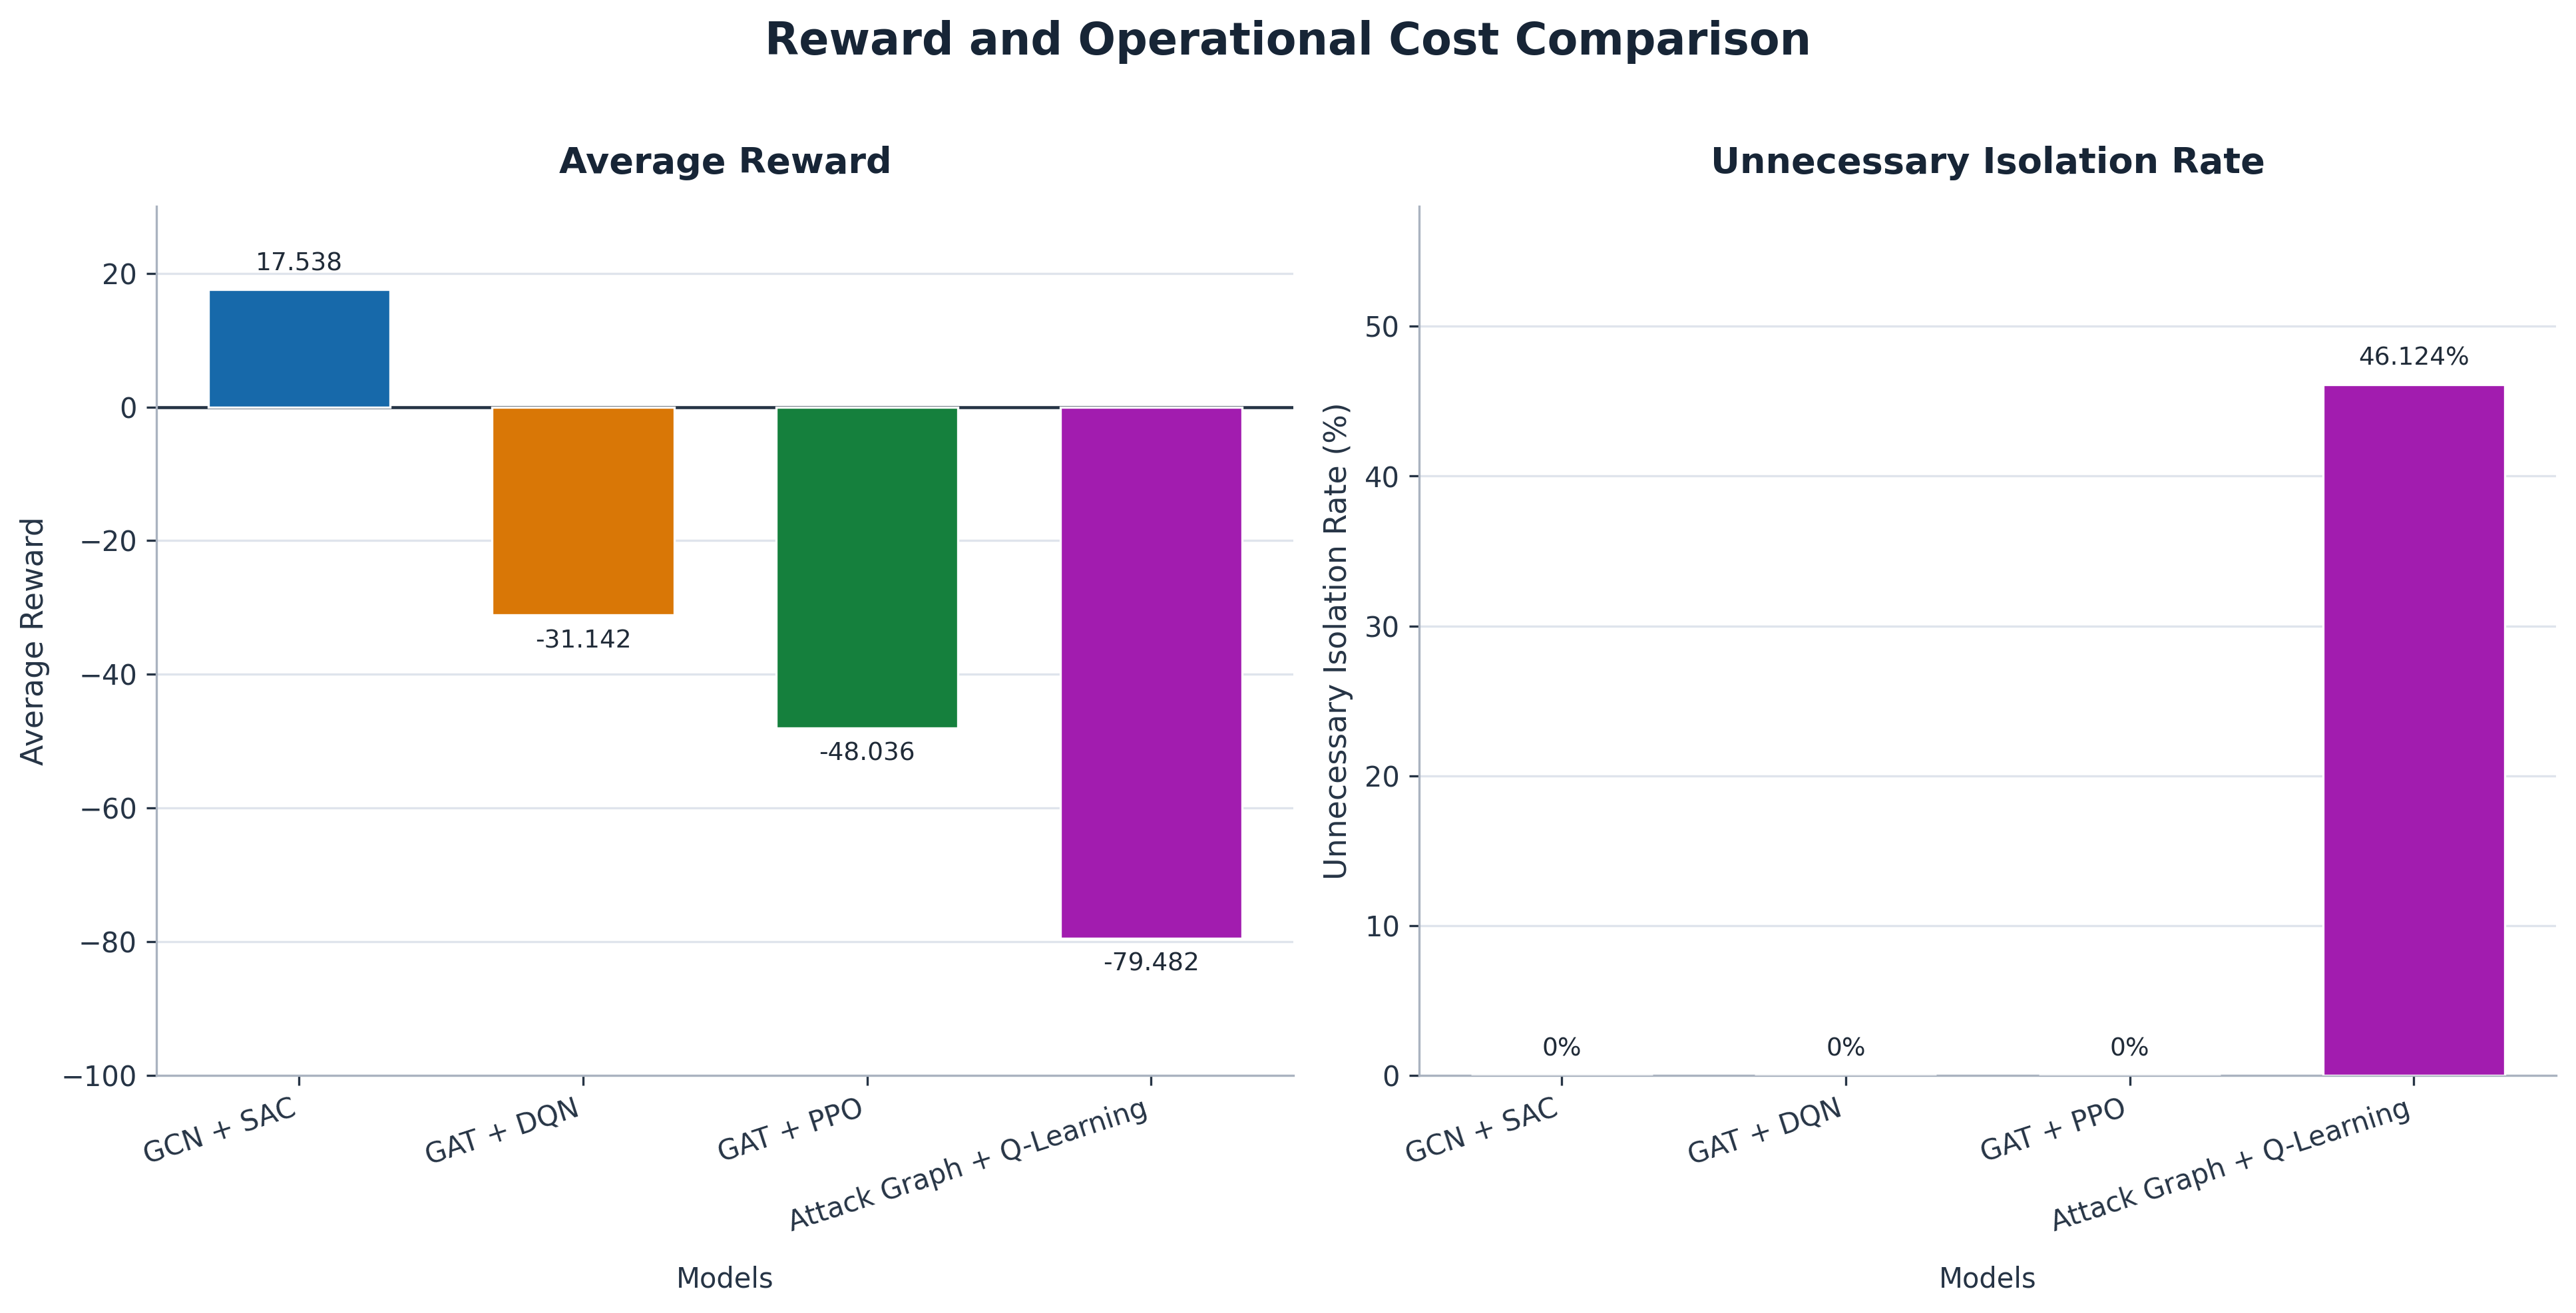
\includegraphics[width=0.98\textwidth]{comparison_charts/05_reward_and_isolation.png}
\caption{Average reward and unnecessary isolation shown on separate axes.}
\label{fig:reward-isolation}
\end{figure}

\section{Result Analysis}

\subsection{Detection Performance}

GCN + SAC leads the reported aggregate accuracy and F1 values. GAT + DQN and GAT + PPO have similar accuracy and F1, while Attack Graph + Q-Learning has the lowest accuracy and F1 but higher precision than the two GAT baselines. Under the current binary decision rule, selecting any non-ALLOW action counts as a positive detection. This makes these measures dependent on defensive action selection and the heuristic target definition, so they should not be described as standalone classifier performance on test records.

\subsection{ROC-AUC}

GCN + SAC has the highest stored ROC-AUC (94.909\%). The other values are 67.415\% for GAT + DQN, 42.620\% for GAT + PPO, and 47.065\% for Attack Graph + Q-Learning. The scoring functions differ by policy type and are not probability-calibrated to a shared detection model. Moreover, the current target incorporates a risk threshold and the compromised state. ROC-AUC should therefore be treated as a comparative diagnostic of these score transformations, not as an independently validated traffic-classification AUC.

\subsection{Defense Performance}

The Q-learning baseline achieves the largest reported defense success and containment percentages. A defense success is not awarded merely for selecting a non-ALLOW action: it must meet the code's resulting-state condition. Containment is likewise based on absence of newly compromised nodes during a defined attack opportunity. These high percentages should be read together with the action costs and isolation rate; they do not imply the best overall policy quality.

\subsection{Attack Reduction}

All four attack-reduction values are negative: -23.810\% for each stored neural-policy baseline and -17.429\% for Q-learning. Thus the final aggregate compromised count exceeds the initial count in all cases. The simulator only changes a node from clean to compromised and does not implement recovery or de-compromise. With that transition design, a positive reduction is not expected; the metric captures additional spread relative to the initial compromised population rather than recovery of compromised nodes.

\subsection{Reward}

GCN + SAC is the only model with positive average episode reward in the current table. Q-learning has the lowest average reward (-79.482), consistent with frequent costly defensive actions and penalties for unnecessary actions. Its high containment result therefore comes with an unfavorable reward/cost trade-off. This is an important example of why containment should not be interpreted without operational cost and reward.

\subsection{Unnecessary Isolation}

The three stored existing-model rows report 0\% unnecessary isolation. Attack Graph + Q-Learning reports 46.124\%, meaning nearly half of its counted isolation actions were applied to nodes not marked compromised before the action. Under the current implementation the unnecessary-isolation numerator is a subset of the isolation-action denominator, so the rate cannot exceed 100\% unless the metric code or its inputs are changed inconsistently.

\section{Overall Model Comparison}

Based on the current stored values, GCN + SAC has the strongest detection-style metrics and positive reward. Attack Graph + Q-Learning has the strongest reported containment and defense success, but also the lowest average reward, the highest unnecessary-isolation rate, and the lowest accuracy/F1. GAT + DQN and GAT + PPO occupy intermediate positions for several detection and reward measures. Because the first three rows are reused historical aggregates and the Q result is separately evaluated, this ranking is descriptive only. It does not establish statistical significance or a controlled architecture-only comparison.

\section{Discussion of Findings}

The results expose a trade-off between containment and operational cost. Q-learning frequently selects strong actions, including isolation and session termination, which aligns with its high containment rate but also with its unnecessary-isolation rate and strongly negative reward. The reward function penalizes defensive operating cost and low-risk intervention, so it distinguishes aggressive containment from cost-aware defense.

The fixed 50-node profile begins with 21 compromised nodes and repeatedly targets the highest-risk node. This creates a constrained simulator scenario and is materially different from evaluating a policy on a held-out collection of independent CSV flow records. In addition, the target used for classification combines compromise status and a risk threshold, while a prediction is defined from the action label. The current detection metrics therefore reflect policy behavior in the simulator, rather than direct generalization to labeled network traffic.

The tabular baseline captures graph-derived risk, node identity, local vulnerability exposure, compromise, isolation, and attack-path distance. However, it treats each node-state/action update using a shared scalar network reward, even though actions are selected simultaneously for all 50 nodes. Its state table is a tractable approximation to a much larger joint action problem. Five training episodes are not enough to establish convergence, and the observed negative reward should be reported as such.

\section{Limitations}

\begin{enumerate}[leftmargin=2em,label=\arabic*.]
  \item \textbf{Mixed-vintage result table:} GCN + SAC, GAT + DQN, and GAT + PPO aggregates are loaded from existing files; only Q-learning was freshly trained/evaluated in the latest run. Evaluation scenario seeds and original run settings for the prior rows are unavailable.
  \item \textbf{Dataset not used for policy evaluation:} \code{combine.csv} is opened for a one-row validation by the comparison runner. The simulator uses hard-coded node features. The comparison is not a row-wise train/test experiment on the CSV.
  \item \textbf{Unrecorded hardware and software provenance:} CPU, memory, checkpoint creation environment, and pinned dependencies are not captured in a run manifest. The versions stated in this chapter describe the current workspace inspection.
  \item \textbf{Small training budget:} Five training episodes are insufficient evidence of convergence for DQN, PPO, or tabular Q-learning. Q-learning in particular explores an extensive state space with only a small number of visits.
  \item \textbf{No uncertainty estimates:} There are no per-seed repetitions, confidence intervals, standard deviations, or hypothesis tests in the result artifacts.
  \item \textbf{Heuristic detection labels:} Targets are derived from pre-action compromise or risk $\geq 0.6$; positive predictions are non-ALLOW defenses. These are not independent labeled predictions on a held-out dataset.
  \item \textbf{Non-comparable score transformations:} ROC-AUC input scores are generated differently by SAC, DQN, PPO, and Q-learning and are not calibrated probabilities.
  \item \textbf{No recovery model:} Compromise propagates but is never cleared, limiting the interpretation of attack reduction and preventing recovery-based positive reductions.
  \item \textbf{Q-learning joint-action approximation:} A common reward is assigned to each per-node state/action pair, and interactions among simultaneous per-node choices are not represented in a joint Q-state/action value.
  \item \textbf{No durable Q checkpoint or run manifest:} The Q-table, exact evaluation seed sequence, per-episode outputs, and configuration are not persisted as a checkpoint alongside the aggregate metrics.
\end{enumerate}

For a stronger final study, run all four models from clean model states against identical saved initial scenarios and random streams, repeat across multiple seeds, persist per-episode records and configuration, use held-out CSV-derived scenarios where appropriate, and report mean and dispersion (or confidence intervals). Any such rerun should be reported as a new experiment rather than silently replacing the current aggregates.

\section{Chapter Summary}

This chapter presented a four-model comparison using the project's 50-node Fat-Tree-like simulator, eight node features, eight defense actions, shared attack routine, and common reward. The current stored table shows GCN + SAC leading detection-style metrics and average reward, while Attack Graph + Q-Learning has the highest containment and defense-success rates but also the most negative average reward and highest unnecessary isolation. All models have negative attack reduction under the no-recovery attack simulator.

The Q-learning implementation uses a tabular Bellman update, epsilon-greedy selection, and node-specific discretized attack-graph states derived from the simulator. The figures display exactly the current aggregates. Interpretation must remain qualified because the table is mixed-vintage, the simulator episodes do not directly draw feature records from \code{combine.csv}, the classification metrics use heuristic targets, and the historical hardware and run provenance are incomplete.

\end{document}